\documentclass[aspectratio=1610]{beamer}
\usepackage[utf8]{inputenc}
\usepackage{multicol}
\usepackage[czech]{babel}
\usepackage{amsmath}
\usepackage{csquotes}

\usepackage[sfdefault]{roboto} 
\usepackage[T1]{fontenc}

\title{Úvodní hodina}
\date{WBA | 1., 2. hodina}
\author[Cajthaml]{Matěj Cajthaml}

\usetheme{material}

\usePrimaryCustom

\begin{document}

\begin{frame}
\titlepage
\end{frame}

\begin{frame}{Obsah prezentace}
    \begin{cardTiny}
        \begin{minipage}{\textwidth}
            \vspace{1ex}
            \tableofcontents
        \end{minipage}
    \end{cardTiny}
\end{frame}



\section{Administrativní záležitosti}

\begin{frameImg}{img/this-is-fine.jpg}
    \vspace*{60mm}
    \begin{cardTiny}
        \vspace*{\fill}
        \begin{center}
            \textbf{Protipožární ochrana}
        \end{center}
    \end{cardTiny}
\end{frameImg}

\begin{frameImg}[height]{img/this-is-fine-art.png}
    \vspace*{60mm}
    \begin{cardTiny}
        \vspace*{\fill}
        \begin{center}
            \textbf{Řád učebny}
        \end{center}
    \end{cardTiny}
\end{frameImg}

\begin{frameImg}[height]{img/sablik.png}
    \vspace*{60mm}
    \begin{cardTiny}
        \vspace*{\fill}
        \begin{center}
            \textbf{Velký Sáblík tě vidí}
        \end{center}
    \end{cardTiny}
\end{frameImg}



\section{O mně}

\begin{frame}{O mně}
    \begin{cardTiny}
        Absolvent Smíchovské SPŠ.
        
        Student Fakulty informačních technologií na ČVUT.

        Nadšenec do webových aplikací.

        Spoluautor nových webových stránek školy.
    \end{cardTiny}
    \begin{cardTiny}
        Kontakt: pomocí e-mailu \texttt{matej.cajthaml@ssps.cz}.

        Používejte oficiální e-mailovou schránku školy.

        Kontrolujte e-mailou schránku a Bakaláře.
    \end{cardTiny}
\end{frame}



\section{O předmětu a hodnocení}

\begin{frame}{O předmětu}
    \begin{multicols}{2}
        \centering
        
        \begin{cardTiny}
            \textbf{Co očekávat}
        
            \begin{flushleft}
            Úvod do webových aplikací.
            
            Responzivní design.

            Základy skriptování.
        
            Úvod do moderních webů.
            \end{flushleft}
        \end{cardTiny}
        
        \begin{cardTiny}
            \textbf{Co neočekávat}
            
            \begin{flushleft}
            Moderní webové stránky.

            Dynamické webové stránky.
            
            Velké peníze beze snahy.

            Že se tady vše naučíte.

            Profesionální návrh webů.
            \end{flushleft}
        \end{cardTiny}
    \end{multicols}
\end{frame}

\begin{frame}{O Vás}
    \begin{cardTiny}
        \textbf{Co očekávám já}
    
        \begin{flushleft}
        Vstřícnost.

        Přátelský přístup.

        Odpovědnost.

        Konstruktivní kritiku.
        \end{flushleft}
    \end{cardTiny}
\end{frame}

\begin{frame}{Pokračování předmětu}
    \begin{cardTiny}
        \textbf{Maturitní VOP}

        Konec druhého ročníku.

        Dynamické a moderní webové stránky.

        Pokročilý design.

        Profesor Marek Kejda.

        3h / týden.
    \end{cardTiny}
\end{frame}

\begin{frameImg}[width]{img/what.png}
    \vspace*{60mm}
    \begin{cardTiny}
        \vspace*{\fill}
        \begin{center}
            \textbf{Kritéria hodnocení}
        \end{center}
    \end{cardTiny}
\end{frameImg}

\begin{frame}{Kritéria hodnocení}
    \begin{cardTiny}
        \begin{flushleft}
            Vlastní poznámky \textbf{nejsou povinné}.

            Všechny písemná zkoušení jsou povinná a musí se dopisovat.

            Je potřeba alespoň 75\% docházky.

            Všechny prezentace, tyto kritéria a další: \href{https://cajthaml.eu/}{https://cajthaml.eu}.
        \end{flushleft}
    \end{cardTiny}
    \begin{cardTiny}
        \textbf{Bodový systém}
            
        \begin{flushleft}
            Nahrazení běžného hodnocení od 1 až 5 za body.

            Body se sčítají celý rok, neresetují se v pololetí.

            Bodový základ tvoří písemné zkoušení a povinné domácí úkoly.

            Spravedlivější systém.

            Podvod je hodnocen zápornými body.
        \end{flushleft}
    \end{cardTiny}
\end{frame}

\begin{frame}{Bodový systém}
    \begin{cardTiny}
        \begin{flushleft}
            Počet bodů za danou práci se přepočítává na známku.

            Známky se zapisují do systému Bakalářů.

            Známky v Bakalářích jsou pouze orientační.

            Aktuální počet bodů a známka: e-mail, po/před hodinou.
        \end{flushleft}
    \end{cardTiny}
    \begin{multicols}{2}
        \centering
        
        \begin{cardTiny}
            \textbf{Body lze získat za:}
        
            \begin{flushleft}
            Písemné zkoušení.

            Ústní zkoušení.

            Povinné úkoly.

            \textbf{Nepovinné úkoly}.

            Závěrečná práce.

            Práce v hodině.
            \end{flushleft}
        \end{cardTiny}
        
        \begin{cardTiny}
            \textbf{Body lze ztratit za:}
            
            \begin{flushleft}
            Namátkové ústní zkoušení.

            Neodevzdané povinné\\~~~úkoly~/~závěrečnou práci.

            Obtěžování v hodině.

            Podvod / lhaní.
            \end{flushleft}
        \end{cardTiny}
    \end{multicols}
\end{frame}

\begin{frame}{Převod bodů na známku}
    \begin{cardTiny}
        \begin{flushleft}
            Z počtu získaných bodů a bodového základu se vypočítá procentuální úspěšnost.

            Podle procentuální úspěšnosti se udělí známka.

            
            
            Ukázka:\\ b. z. = 35, z. b. = 29  tedy  $\frac{29}{35} \times 100 = 82.8\% \to \textbf{2}$
        \end{flushleft}
    \end{cardTiny}
    \begin{cardTiny}
        \begin{center}
            \begin{tabular}{ |c|c| } 
                \hline
                $<$ 40\% & 5 \\ 
                40\% - 55\% & 4 \\ 
                55\% - 70\% & 3 \\ 
                70\% - 85\% & 2 \\ 
                $\geq$ 85\% & 1 \\ 
                \hline
            \end{tabular}
        \end{center}
    \end{cardTiny}
\end{frame}

\begin{frame}{Závěrečná práce}
    \begin{cardTiny}
        \begin{flushleft}
            Práce na druhé pololetí.
            
            Vytvoření práce - webových stránek na dané téma dle požadavků.

            Práce se prezentuje před třídou kdykoliv v druhém pololetí, nejpozději měsíc před klasifikací.
            
            \vspace{2ex}
            75\% bodů za samostatnou práci, 25\% za prezentaci.
        \end{flushleft}
    \end{cardTiny}
\end{frame}

\begin{frame}{Průběh hodiny}
    \begin{cardTiny}
        \begin{flushleft}
            Absence.

            Opakování z minulých hodin.

            Látka.

            Opakování hodiny.
        \end{flushleft}
    \end{cardTiny}
    \begin{cardTiny}
        \begin{flushleft}
            Otázky.

            Toaleta.

            Přestávky.
        \end{flushleft}
    \end{cardTiny}
\end{frame}

\begin{frame}{Co nás čeká}
    \begin{cardTiny}
        \begin{flushleft}
            Teorie internetu, webových stránek.

            Bezpečnost na internetu, prohlížeče, autorský zákon.
            
            \textbf{Test č. 1}.

            Základy HTML.

            Základy CSS.

            ...
        \end{flushleft}
    \end{cardTiny}
\end{frame}

\begin{frameImg}[width]{img/uno.jpg}
    \vspace*{60mm}
    \begin{cardTiny}
        \vspace*{\fill}
        \begin{center}
            \textbf{Teď vy!}
        \end{center}
    \end{cardTiny}
\end{frameImg}


\section{Internet}

\begin{frameImg}[width]{img/internet.jpg}
    \vspace*{60mm}
    \begin{cardTiny}
        \vspace*{\fill}
        \begin{center}
            \textbf{Internet}
        \end{center}
    \end{cardTiny}
\end{frameImg}

\begin{frame}{Internet}
    \begin{cardTiny}
        \begin{flushleft}
            Internet = celosvětový systém navzájem propojených počítačových sítí.

            
            \vspace{2ex}
            Počítačová síť = sdružení technických prostředků, realizující spojení a výměnu informací.

            
            \vspace{2ex}
            Typy počítačových sítí: \textbf{peer to peer} a \textbf{client server}.
        \end{flushleft}
    \end{cardTiny}
\end{frame}


\begin{frame}
    \begin{center}    
        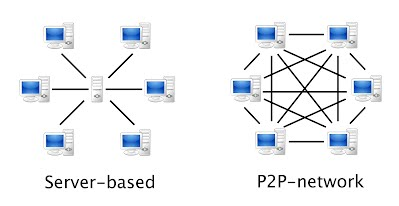
\includegraphics[width=0.8\textwidth]{img/p2pcs.jpg}
    \end{center}

    \begin{cardTiny}
        \begin{center}
            \textbf{Jaké služby využívají internet?}
        \end{center}
    \end{cardTiny}
\end{frame}

\begin{frame}{Služby využívající Internet}
    \begin{cardTiny}
        \begin{center}
            Webové stránky, e-mail, komunikace, přenos videa a zvuku, sdílení souborů, ...
        \end{center}
    \end{cardTiny}
    \begin{cardTiny}
        \begin{flushleft}
        \begin{center}
            \textbf{Jaké existují počítačové sítě?}
        \end{center}
        \end{flushleft}
    \end{cardTiny}
\end{frame}

\begin{frame}{Počítačové sítě}
    \begin{cardTiny}
        \begin{center}
            Vědecké, vojenské, bankovní instituce.

            Vysoké školy.

            Osobní (soukromé) domácí sítě.
        \end{center}
    \end{cardTiny}
\end{frame}

\begin{frame}{Historie internetu}
    \begin{cardTiny}
        \begin{flushleft}
            Point-to-point internet po 2. světové válce.

            1969 vznikla síť ARPANET s 4 uzly.

            1972 byla síť ARPANET připojena na cca 70 zařízení.

            Následovaly další sítě, které se navzájem připojovaly.

            Dnešní internet jsou sítě propojené po celém světě.

            1992 ČVUT se připojilo k internetu (Rakousko, Linec).
        \end{flushleft}
    \end{cardTiny}
    \begin{cardTiny}
        \begin{center}
            \begin{tabular}{ |c|c| } 
                \hline
                1978 & 27 tisíc zařízení        \\
                1996 & 55 milionů zařízení      \\
                2000 & 250 milionů zařízení     \\
                2009 & 1.8 miliardy zařízení    \\
                \hline
            \end{tabular}
        \end{center}
    \end{cardTiny}
\end{frame}

\begin{frame}
    \begin{center}
    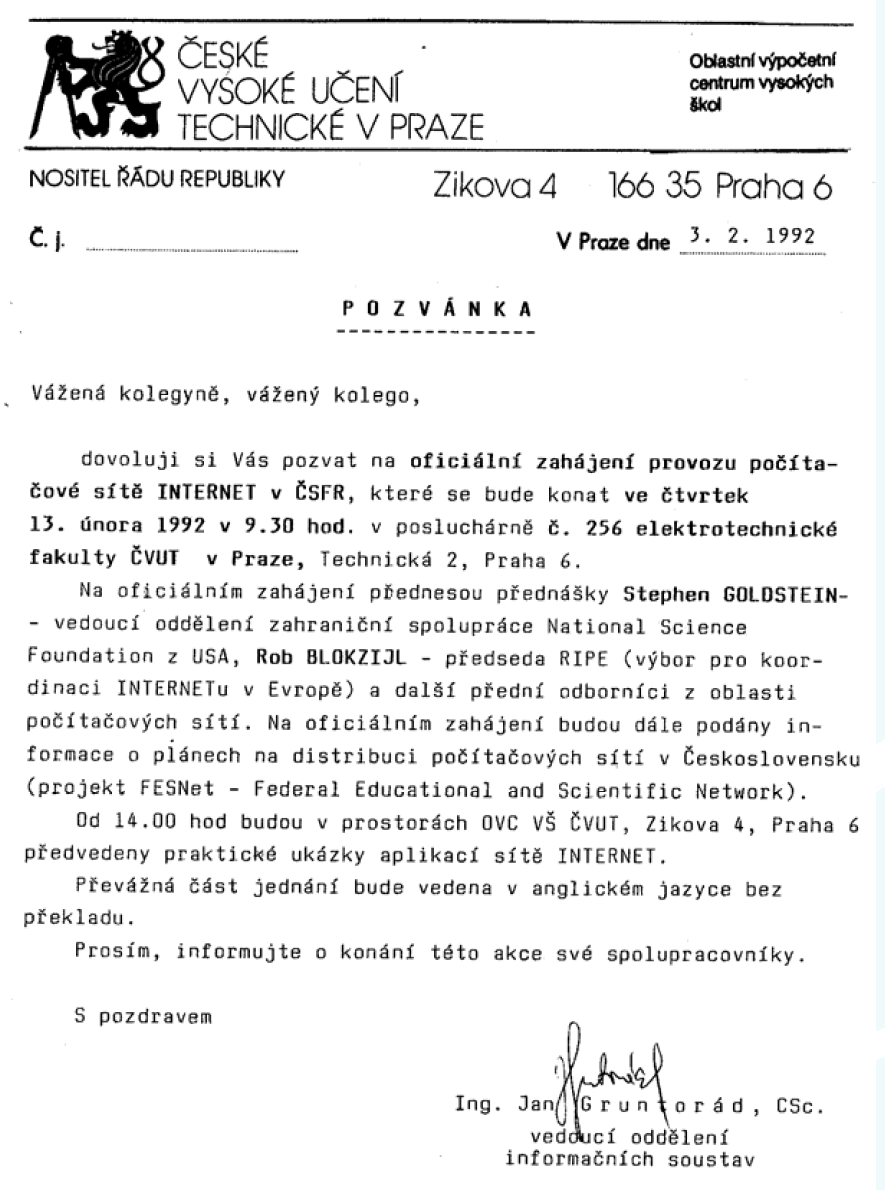
\includegraphics[width=0.4\textwidth]{img/cvut.png}
    \end{center}
\end{frame}

\section{World Wide Web}

\begin{frameImg}[width]{img/web.jpg}
    \vspace*{60mm}
    \begin{cardTiny}
        \vspace*{\fill}
        \begin{center}
            \textbf{World Wide Web - WWW}
        \end{center}
    \end{cardTiny}
\end{frameImg}

\begin{frame}{World Wide Web}
    \begin{cardTiny}
        \begin{flushleft}
            WWW = soustava propojených \textbf{hypertextových dokumentů}.

            \vspace{2ex}
            Hypertextový dokument = dokument, který je vázán \textbf{hyperlinky} na jiné dokument.

            Hypertextový dokument není strukturově lineární.

            \vspace{2ex}
            Pro zobrazení je potřebný \textbf{webový prohlížeč}.

            \vspace{2ex}
            Dokumenty jsou přenášeny pomocí protokolu \textbf{HTTP(S)} ve formátu \textbf{HTML}.

            \vspace{2ex}
            Dokumenty se adresují pomocí \textbf{URL}.
        \end{flushleft}
    \end{cardTiny}
\end{frame}

\begin{frame}{Doména}
    \begin{cardTiny}
        \begin{flushleft}
        Doména = jednoznačné jméno (tedy identifikátor) serveru na internetu.

        Posloupnost několik částí oddělených tečkami.

        ASCII, ignoruje velikost písmen. 
        \end{flushleft}
    \end{cardTiny}
    
    \begin{multicols}{2}
        \centering
        
        \begin{cardTiny}
            \textbf{Doména 1. řádu}
        
            \begin{flushleft}
                Určuje zemi / obecnou skupinu.

                Např. \textbf{.cz}, \textbf{.uk}, \textbf{.fr}
            \end{flushleft}
        \end{cardTiny}

        \begin{cardTiny}
            \textbf{Doména x. řádu:}
            
            \begin{flushleft}
            Tzv. subdoména - poddoména

            Např. \textbf{email}.seznam.cz
            \end{flushleft}
        \end{cardTiny}
        
        \begin{cardTiny}
            \textbf{Doména 2. řádu:}
            
            \begin{flushleft}
            Nejčastější případ koupě.

            Určuje společnost / entitu.

            Např. \textbf{seznam}.cz
            \end{flushleft}
        \end{cardTiny}
    \end{multicols}
\end{frame}

\begin{frame}{URL adresa}
    \begin{cardTiny}
        \begin{flushleft}
            Řetězec znaků s definovanou strukturou.

            \vspace{2ex}
            URL = Uniform Resource Locator

            Specifické umístění souboru na internetu a serveru.

            Záleží na velikosti písmen, vyjma protokolu a domény.

            (Ne)poviné části.
        \end{flushleft}
    \end{cardTiny}
    \begin{cardTiny}
        \begin{center}
            $ \overbrace{\text{https:/}}^{\text{protokol}}
            \overbrace{\text{/ssps.cz}}^{\text{doména}}
            \overbrace{\text{:443/}}^{\text{port}}
            \overbrace{\text{o-skole/pedagogicky-sbor.html}}^{\text{umístění na serveru}}
            \overbrace{\text{?p=1}}^{\text{parametry}}
            \overbrace{\text{\#seznam}}^{\text{kotva}} $
        \end{center}
    \end{cardTiny}
\end{frame}

\begin{frame}{Určete části URL} 
    \begin{cardTiny}
        \begin{center}
            $ \overbrace{\text{https://}}^{\text{ }}
            \overbrace{\text{en.wikipedia.org/}}^{\text{ }}
            \overbrace{\text{wiki/IPv6/}}^{\text{ }}
            \overbrace{\text{\#Security}}^{\text{ }} $
        \end{center}
    \end{cardTiny}
\end{frame}

\begin{frame}{Platné URL}
    \begin{cardTiny}
        \begin{flushleft}
            $ \text{https://cs.wikipedia.org/wiki/Česko} $

            $ \text{https://www.jakpsatweb.cz/html/url.html} $

            $ \text{https://www.luxor.cz/checkout/delivery\_and\_payment} $

            $ \text{https://ssps.cz/news/read/452} $

            $ \text{https://www.presloviny.cz/kategorie/technologie/} $

            $ \text{https://www.postovnisporitelna.cz/portal/ucty/postovni-ucet} $
        \end{flushleft}
    \end{cardTiny}
\end{frame}


\begin{frame}{URL adresy}
    \begin{cardTiny}
        \begin{center}
            \textbf{ÚKOL}
        \end{center}
        \begin{flushleft}
            Vyzkoušejte různé URL adresy, protokoly s různými kotvami a parametry, procházejte známe webové stránky a zjistěte, jak jejich URL vypadají.

            \vspace{2ex}            
            Narazili jste na něco speciálního? Jaké stránky jste zkoušeli?

            Existuje neplatná URL?

            Přečtěte (vyhledejte) si stránku "What is URL?"~ na stránce \\~~~developer.mozilla.org. Co nového jste se dozvěděli?
        \end{flushleft}
    \end{cardTiny}
\end{frame}

\begin{frame}{Webový vyhledávač}
    \begin{cardTiny}
        \begin{flushleft}
            Automatický systém vyhledávající informace na WWW.

            Podobnost s tzv. \href{https://odkazy.seznam.cz}{\textbf{webovým katalogem}}.

            Vypnutí pomocí souboru robots.txt.

            \href{https://en.wikipedia.org/wiki/List\_of\_search\_engines}{ODKAZ - Seznam webových vyhledávačů}

            Hluboký web (deep web) / Temný web (dark web).
        \end{flushleft}
    \end{cardTiny}
    \begin{cardTiny}
        \begin{center}
            \textbf{Kam patří virtuální škola, Bakaláři, web školy, E-mailový klient?}
        \end{center}
    \end{cardTiny}
\end{frame}

\begin{frame}
    \begin{center}
        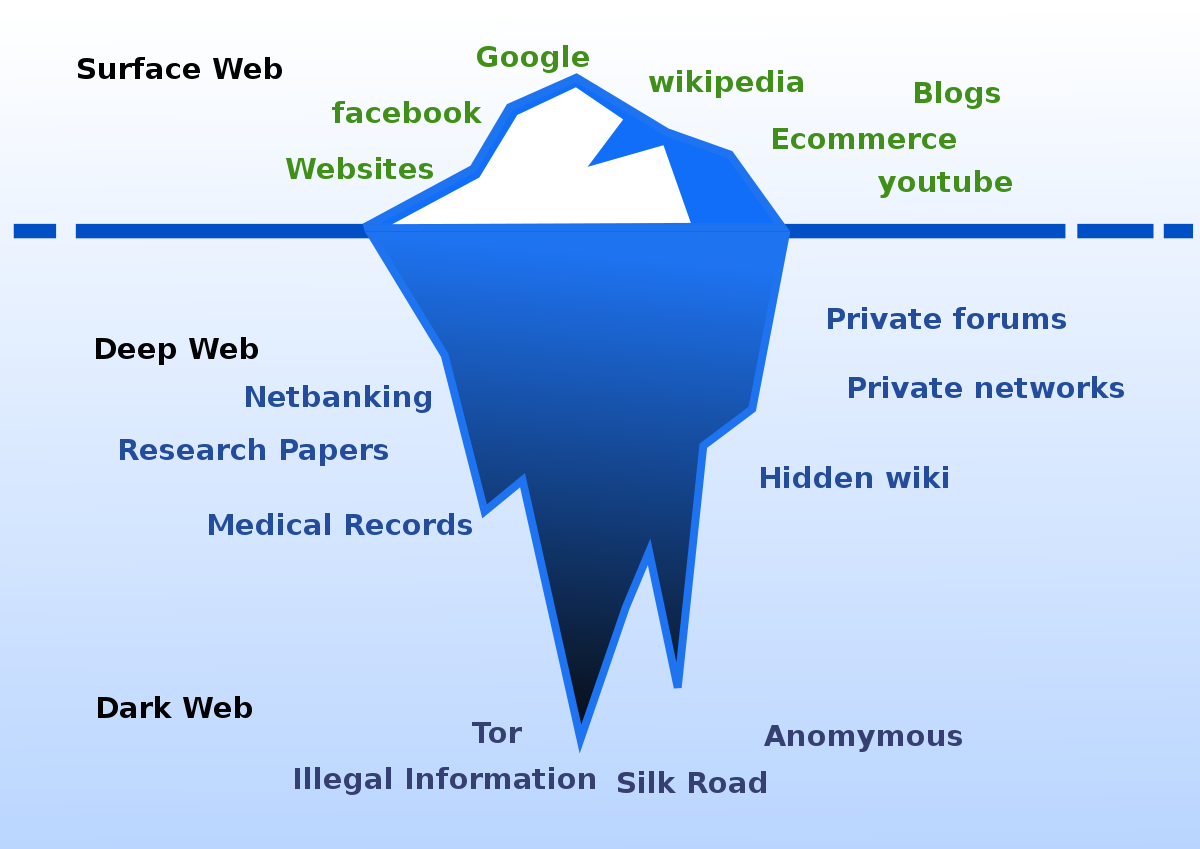
\includegraphics[width=0.8\textwidth]{img/dwdwwww.jpg}
    \end{center}
\end{frame}



\section{Webové protokoly}
\begin{frame}{Webové protokoly}
    \begin{cardTiny}
        \begin{center}
            Existuje nespočet webových protokolů.

            Každý protokol si určuje vlastní syntaxi, sémantiku a synchronizaci.
        \end{center}
    \end{cardTiny}
\end{frame}

\begin{frame}
    \begin{multicols}{2}
        \centering
        
        \begin{cardTiny}
            \textbf{HTTP}
        
            \begin{flushleft}
            = Hyper Text Transfer Protocol

            \vspace{2ex}
            Přenos hypertextových dokumentů.

            Obyčejně se využívá port 80.
            
            \vspace{2ex}
            Dnes je základem pro mnoho odvětví v IT.
            \end{flushleft}
        \end{cardTiny}

        \begin{cardTiny}
            \textbf{HTTPS}
            
            \begin{flushleft}
            = HTTP \textbf{Secure}

            \vspace{2ex}
            Zabezpečená nástavba HTTP.
            
            Data jsou šifrována.

            Obyčejně se využívá port 443.
            
            \vspace{2ex}
            Dříve používán pro přenos důvěrných informací.

            Dnes je nutný skoro na všech webových stránkách.
            \end{flushleft}
        \end{cardTiny}
    \end{multicols}
\end{frame}

\begin{frame}
    \begin{multicols}{2}
        \centering
        

        \begin{cardTiny}
            \textbf{IP}
            
            \begin{flushleft}
            = Internet Protocol

            \vspace{2ex}
            Směrování na internetu.

            Směrování packetů.

            Síťová vrstva.

            \vspace{2ex}
            IPv4 je \textbf{vyčerpaná}.

            \vspace{2ex}
            IPv4 $\rightarrow$ \texttt{192.168.0.1}

            IPv6 $\rightarrow$ \texttt{2001:718::fec9:ca5}
            \end{flushleft}
        \end{cardTiny}

        \begin{cardTiny}
            \textbf{DNS}
        
            \begin{flushleft}
            = Domain Name System

            \vspace{2ex}
            Převod doménových jmen na IP.
            
            \vspace{2ex}
            Hierarchický systém.

            Lepší orientace pro lidi.

            \vspace{2ex}
            \texttt{seznam.cz} převede na \texttt{77.75.76.3}.

            \end{flushleft}
        \end{cardTiny}
    \end{multicols}
\end{frame}


\begin{frame}{IP adresy}
    \begin{cardTiny}
        \begin{center}
            \textbf{ÚKOL}
        \end{center}
        \begin{flushleft}
            Nalezněte vaší IP adresu. Určete v jakém formátu je. Je unikátní ve třídě?
        \end{flushleft}
    \end{cardTiny}
\end{frame}


\begin{frame}
    \begin{center}
    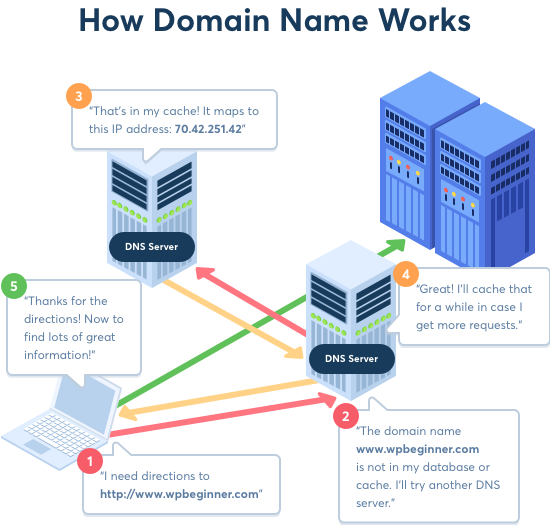
\includegraphics[width=0.6\textwidth]{img/dns.png}
    \end{center}
\end{frame}

\begin{frame}
    \begin{cardTiny}
        \textbf{FTP}
        
        \begin{flushleft}
            = File Transfer Protocol

            \vspace{2ex}
            Přenášení souborů mezi počítači.

            Různé operace.

            \vspace{2ex}
            FTP klient.

            FTP v prohlížeči.

            \vspace{2ex}
            Využívá model klient-server.

            Např. nahrávání webových stránek, zalohování.

            Např. WINScp, FreeCommander, ...
        \end{flushleft}
    \end{cardTiny}
\end{frame}

\begin{frame}
    \begin{center}
    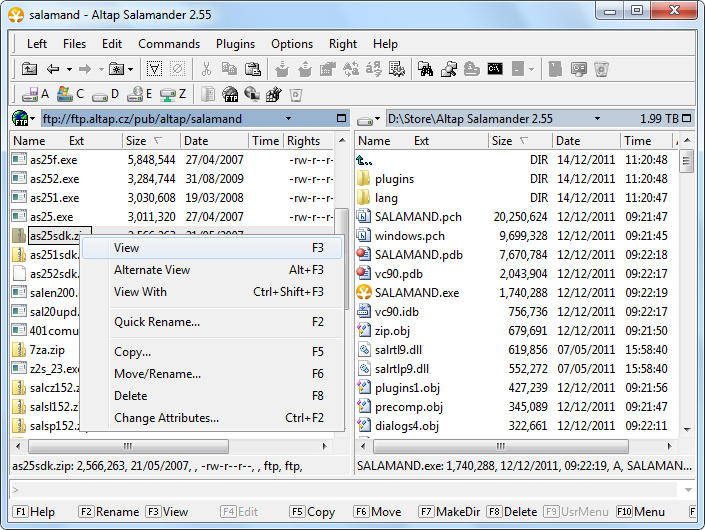
\includegraphics[width=0.8\textwidth]{img/ftp.png}
    \end{center}
\end{frame}



\begin{frame}{IP adresy}
    \begin{cardTiny}
        \begin{center}
            \textbf{ÚKOL}
        \end{center}
        \begin{flushleft}
            Sepiště v pěti bodech zajímavé informace o nějakém dalším protokolu.
        \end{flushleft}
    \end{cardTiny}
\end{frame}



\section{Shrnutí}
\begin{frame}{Shrnutí}
    \begin{cardTiny}
        \begin{center}
            \textbf{Co je to Internet a počítačová síť?}
        \end{center}
    \end{cardTiny}

    \begin{cardTiny}
        \begin{center}
        \textbf{Jaký je rozdíl mezi HTTP a HTTPS?}
        \end{center}
    \end{cardTiny}

    \begin{cardTiny}
        \begin{center}
        \textbf{Co je to URL?}
        \end{center}
    \end{cardTiny}

    \begin{cardTiny}
        \begin{center}
        \textbf{Co to je DNS?}
        \end{center}
    \end{cardTiny}

    \begin{cardTiny}
        \begin{center}
        \textbf{Jaký rozdíl je mezi webovým katalogem a vyhledávačem?}
        \end{center}
    \end{cardTiny}
\end{frame}

\end{document}